%%%%%%%%%%%%%%%%%%%%%%%%%%%%%%%%%%%%%%%%%%%%%%%%%
%       Client                                  %
%                                               %
%%%%%%%%%%%%%%%%%%%%%%%%%%%%%%%%%%%%%%%%%%%%%%%%%
\subsection{Client} % Interface Client
\begin{figure}[H]
\centering
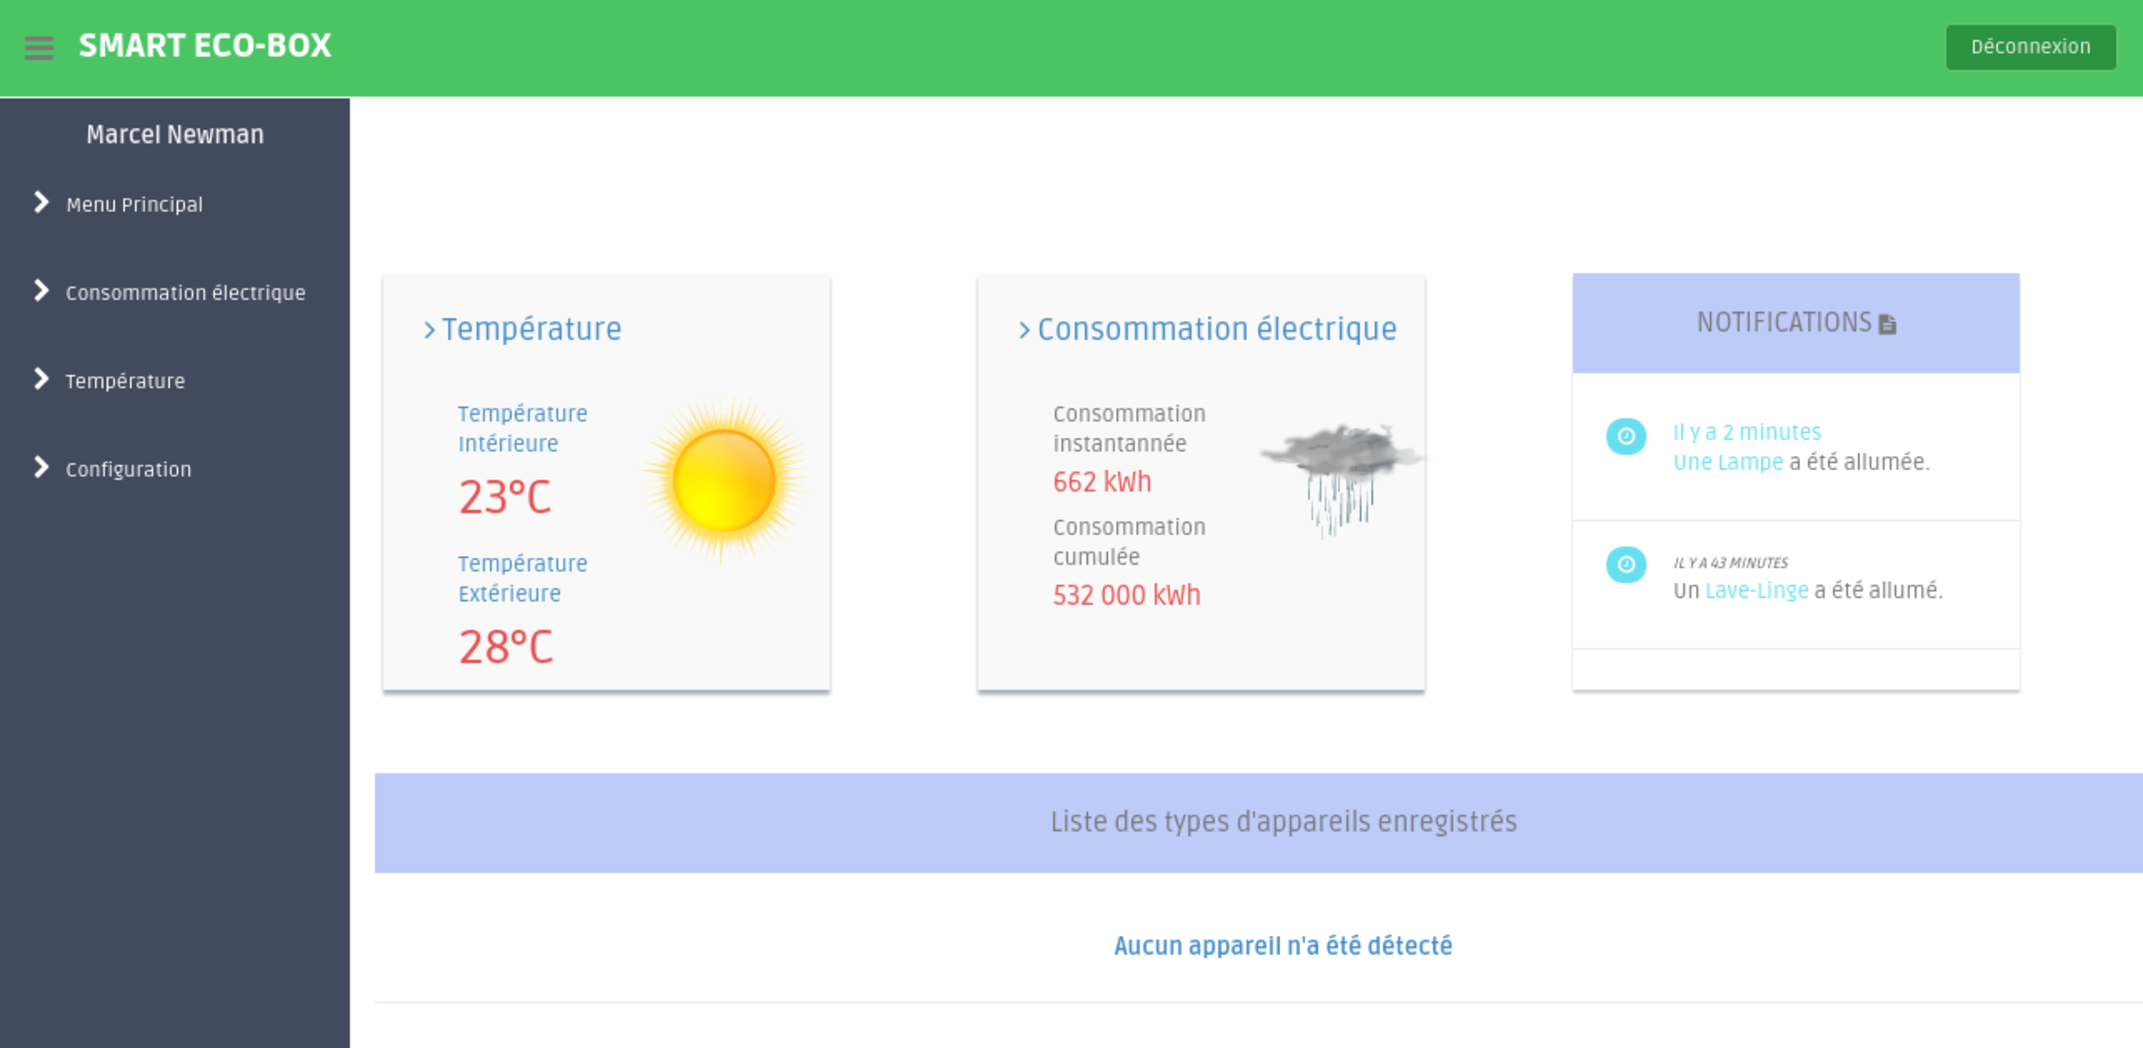
\includegraphics[scale=0.4]{figures/Accueil.pdf}
\caption{Homepage of the webapp}
\label{fig:Accueil}
\end{figure}
This subsection introduces the design of the web interface, especially the structure and the implementation of the main features.
% expliquer l'utilité de l'interface

%%%%%%%%%%%%%%%%%%%%%%%%%%%%%%%%%%%%%%%%%%%%%%%%%%%%%%%%%%%%%%%%%%%%%%%%%%%%%
\subsubsection{Structure}
    % serveur léger -> traitement côté client -> JS -> Angular
    % parler MVC avec Angular
    % n3-chart : n3-chart makes creating beautiful charts for AngularJS application easy and semantic. It is built on top of D3.js library.
    %
    % schéma du site
    Given that the server has to be light and has only to provide the data, this interface has been built with the framework AngularJS 1.3. Indeed, it enables efficient and easily maintainable client-side data processing. In addition, it is based on the Model-View-Controller architectural pattern (MVC) that allows easy maintenance of the code. The curves have been built with the n3-chart library. It makes creating beautiful charts for AngularJS application easy and semantic and it is built on top of D3.js library.
    
    The interface has four main pages reachable via the navigation bar: Homepage, Power Consumption page, Temperature page and the Configuration page. Besides, the login page to access the web app and the page to set up and configure the box are designed.
     
    \begin{figure}[!h] 
        \centering
        % pour changer la couleur
        %%  cf main.tex à \tikzstyle pour tout le document
        %   ou
        %%  cf webapp.tex pour savoir comment changer la couleur d'un node
        \begin{tikzpicture}[node distance=1.5cm]
    
        \node (startConf) [startstop] {Setting up and Configuring};
        \node (login) [process, below of=startConf] {Log in};
        \node (home) [process, below of=login] {Homepage};
        \node (conf) [process, below of=home] {Configuration};
        \node (conso) [process, right of=conf, xshift=2cm] {Power Consumption};
        \node (temp) [process, left of=conf, xshift=-2cm] {Temperature};

        \draw [arrow] (startConf) -- (login);
        \draw [arrow] (login) -- (home);
        \draw [arrow] (home) -- (conf);
        \draw [arrow] (home) -- (conso);
        \draw [arrow] (home) -- (temp);
        \end{tikzpicture}
    \end{figure}

     
%%%%%%%%%%%%%%%%%%%%%%%%%%%%%%%%%%%%%%%%%%%%%%%%%%%%%%%%%%%%%%%%%%%%%%%%%%%%%
\subsubsection{Homepage}

The homepage provides quick access to the general state of the system.
The main information related to the system's operation and an overview of the data sent by the sensors can be found on this page.
The homepage includes four main blocks:%, - one for electric consumption and one for temperature, one for notifications and one for the states of registered devices - where the most important data will be indicated.
    \paragraph{Power Consumption} 
    This block provides acces to two types of information: the instantaneous and accumulated power consumptions of the house. An icon related to the theme of meteorology indicates the evolution of these data. % TODO Button to switch and see the cost
    \paragraph{Temperature}
    This block provides acces to two main information: inside and outside temperatures.
    \paragraph{Notifications}
    This block enables the user to monitor changes of sensor statuses and registered types of device statuses.The system notifies the user when a status changes.
    %State sensor
    %State registered devices
    \paragraph{List of Devices} % Liste des types d’appareils enregistrés
    This block provides access to all registered types of devices and their statuses.
    %know the state of all registered type of devices.

%%%%%%%%%%%%%%%%%%%%%%%%%%%%%%%%%%%%%%%%%%%%%%%%%%%%%%%%%%%%%%%%%%%%%%%%%%%%%
\subsubsection{Power Consumption}

    \paragraph{Curve Page}
    % suivre evolution de sa conso
    %   courbe de conso
    %   courbe de coût associé
    %   coût cumulé sur la période.
    The user can access the evolution of his domestic power consumption thanks to three elements of information: the power consumption curve, the matched cost curve and the accumulated cost.
    
    \paragraph{Estimated Electricity Bill}
    An estimated electricity bill can be viewed on this page. It is inspired by a real electricity bill and allows the user to know an estimate depending on his behaviour.
%%%%%%%%%%%%%%%%%%%%%%%%%%%%%%%%%%%%%%%%%%%%%%%%%%%%%%%%%%%%%%%%%%%%%%%%%%%%%
\subsubsection{Temperature}
    % suivre evolution de la temperature au sein sa maison
    %   courbes de temperature
    %   plusieurs capteurs
    For each temperature sensor, a temperature curve can be displayed allowing the user to access the evolution of the temperature within the house. 
%%%%%%%%%%%%%%%%%%%%%%%%%%%%%%%%%%%%%%%%%%%%%%%%%%%%%%%%%%%%%%%%%%%%%%%%%%%%%
\subsubsection{Configuration Pages}
    
    \paragraph{Setting up and Configuring} % configuration à l'allumage
    
    When the user turns on his box for the first time, he needs to register by providing his personal data: name, email, password, city, and his EDF subscription. Then, the system automatically displays the different sensors detected thanks to the signal processing algorithm. The user has to set up the system by providing the name, the location and the type of each sensor. % (a color-based recognition could be used)
    
    \paragraph{Current Usage} % pendant l'utilisation
    
    \subparagraph{"My Account" Page:} 
    The user can access his personal information and change it. This includes his name, password, email, city and his EDF subscription. Similarly, the profile appears on the homepage.
    
    \subparagraph{"My Sensors" Page:}
    This page is used to list the different sensors. Each sensor can be renamed by the user, may indicate a location specified by the user (eg children's room) and also specifies a type of sensor that is recognized by a color code. Besides, the SNR (Signal-to-Noise Ratio) is indicated as the form of bars to show the state of a sensor (like mobile phone signal bars). Finally, the user can edit the sensor information using the "Edit" button.